\documentclass[fleqn]{article}
\oddsidemargin 0.0in
\textwidth 6.0in
\thispagestyle{empty}
\usepackage{import}
\usepackage{amsmath}
\usepackage{graphicx}
\usepackage{flexisym}
\usepackage{calligra}
\usepackage{amssymb}
\usepackage{bigints} 
\usepackage[english]{babel}
\usepackage[utf8x]{inputenc}
\usepackage{float}
\usepackage[colorinlistoftodos]{todonotes}


\DeclareMathAlphabet{\mathcalligra}{T1}{calligra}{m}{n}
\DeclareFontShape{T1}{calligra}{m}{n}{<->s*[2.2]callig15}{}
\newcommand{\scriptr}{\mathcalligra{r}\,}
\newcommand{\boldscriptr}{\pmb{\mathcalligra{r}}\,}

\definecolor{hwColor}{HTML}{442020}

\begin{document}

  \begin{titlepage}

    \newcommand{\HRule}{\rule{\linewidth}{0.5mm}}

    \center

    \begin{center}
      
\includegraphics[height=11cm, width=11cm]{asu.png}
    \end{center}

    \vline

    \textsc{\LARGE Statistical/Thermal Physics}\\[1.5cm]

    \HRule \\[0.5cm]
    { \huge \bfseries Quiz 12}\\[0.4cm] 
    \HRule \\[1.0cm]

    \textbf{Behnam Amiri}

    \bigbreak

    \textbf{Prof: Michael Treacy}

    \bigbreak

    \textbf{{\large \today}\\[2cm]}

    \vfill

  \end{titlepage}

  
  By signing my name, I am promising that I did this quiz on my own without any outside help.

  \vspace{0.5cm}

  Name: \textbf{Behnam Amiri}

  \vspace{1cm}

  Consider a system of five particles in a container with \textbf{evenly-spaced energy levels} (e.g. a $1D$ 
  harmonic-oscillator potential).
  In this problem you will consider the allowed energy states of the system. These will depend on
  whether the particles are $(i)$ \textbf{distinguishable particles, } $(ii)$ \textbf{indistinguishable bosons}
  or $(iii)$ \textbf{indistinguishable fermions.}
  To depict the energy levels, we shall use a notation
  $$
    v ~ w ~ x ~ y ~ z ~ ... ~ (d)
  $$
  with $v$ being the number of particles in the lowest energy level; $w$ being the number of particles
  occupying the next-highest energy level, and so on. This is the notation used in the lecture. The
  number $d$ is an additional detail and it represents the degeneracy of the state (i.e. the number of
  \emph{distinguishable} ways of arranging the same state). In this question, ignore the "up"/"down" spin
  possibilities of fermions.

  \pagebreak

  \begin{enumerate}
    \item (7 points) Choose the answer that correctly gives the ground state for each of these cases:
    \begin{center}
      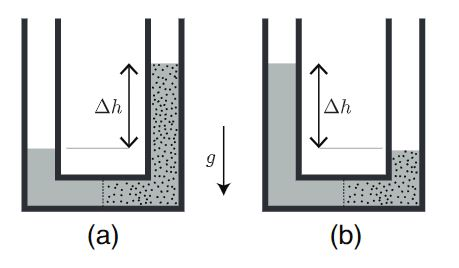
\includegraphics[height=10cm, width=15cm]{1.JPG}
    \end{center}

      \textcolor{hwColor}{
        Note that Fermions \textbf{cannot occupy} the same state but they are
        \textbf{allowed} for Bosons.
        \\
        \\
        \textbf{Bosons} have integer spins, $0,1,2,... ~~~~ \hbar$ units
        \\
        \\
        \textbf{Fermions} have half-integer spins, $\dfrac{1}{2}, \dfrac{3}{2},... ~~~ \hbar$ units.
        \\
        For distinguishable particles or bosons, all five particles occupy the lowest 
        energy level with ground state given by $5 ~ 0 ~ 0 ~ 0 ~ 0$. For fermions. no more than 
        one particle can occupy each energy level with ground state, $1 ~ 1 ~ 1 ~ 1 ~ 1$. Hence, option 
        $(g)$ is correct.
      }
      \begin{center}
        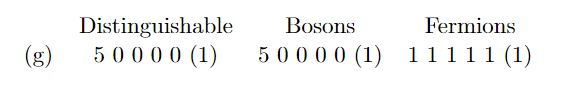
\includegraphics[height=2cm, width=12cm]{Answer1.JPG}
      \end{center}

    \pagebreak

    \item (7 points) Suppose that the system has one unit of energy added to it, raising the system above
    the ground state. Choose the answer below that describes correctly the states of the three
    systems:
    \begin{center}
      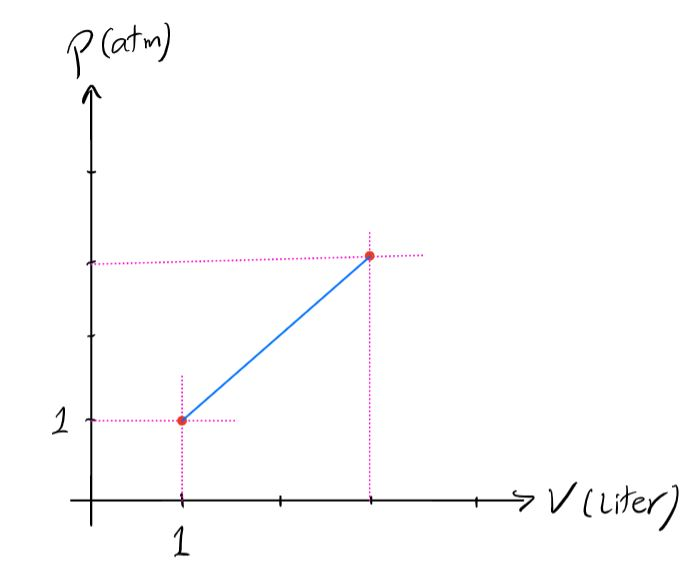
\includegraphics[height=10cm, width=15cm]{2.JPG}
    \end{center}

      \textcolor{hwColor}{
        For distinguishable particles or bosons, one particles goes to the next level. Nore that there are $5$ different ways of doing this for distinguishable particles.
        Fermions' energy levels is $1 ~ 1 ~ 1 ~ 1 ~ 0 ~ 1$. Hence, option $(f)$ is correct.
      }
      \begin{center}
        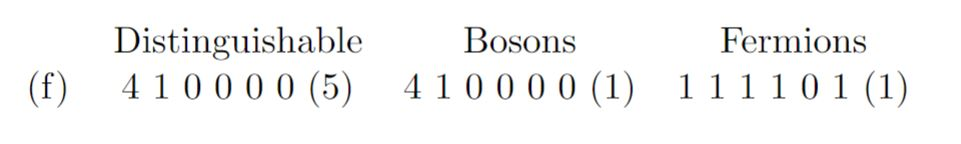
\includegraphics[height=2cm, width=12cm]{Answer2.JPG}
      \end{center}

    \pagebreak

    \item (7 points) We repeat part (2) but there are now two units of energy added. Choose the answer
    below that describes correctly the states of the three systems:
    \begin{center}
      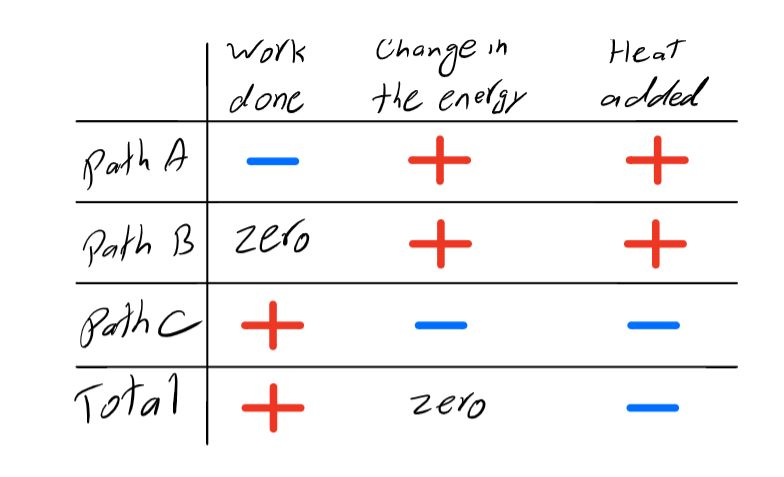
\includegraphics[height=11cm, width=15cm]{3.JPG}
    \end{center}

      \textcolor{hwColor}{
        I am  a bit doubtful about this. Option $e$ seems correct to me but I still go with option $(c)$.
      }
      \begin{center}
        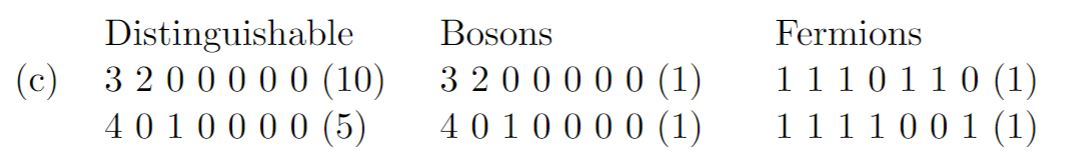
\includegraphics[height=2cm, width=12cm]{Answer3.JPG}
      \end{center}

    \pagebreak

    \item (1 point each) Each system is now given $3$ units of energy. The possible states are presented
    below. Give the degeneracies of each state, i.e. give the nine values $D_1, D_2, D_3, B_1, B_2, B_3,
    F_1, F_2$ and $F_3$.
    \begin{center}
      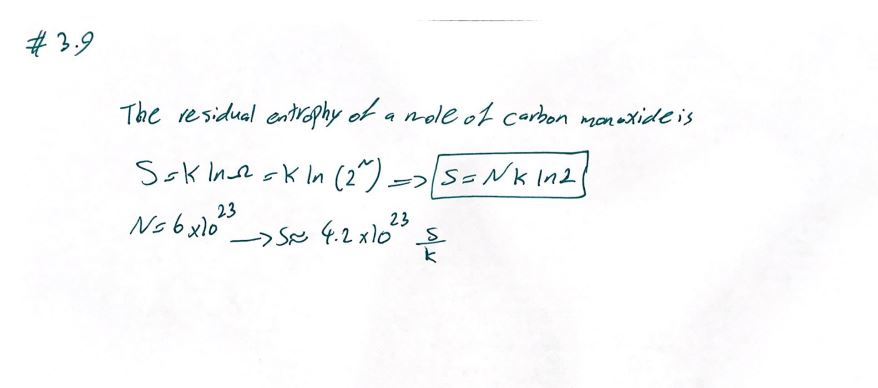
\includegraphics[height=3cm, width=11cm]{4.JPG}
    \end{center}

    $
      D_1=
      \\
      \\
    $

    $
      D_2=
      \\
      \\
    $

    $
      D_3=
      \\
      \\
    $

    $
      B_1=
      \\
      \\
    $

    $
      B_2=
      \\
      \\
    $

    $
      B_3=
      \\
      \\
    $

    $
      F_1=
      \\
      \\
    $

    $
      F_2=
      \\
      \\
    $

    $
      F_3=
      \\
      \\
    $
    
  \end{enumerate}

\end{document}
